%%%%%%%%%%%%%%%%%%%%%%%%%%%%%%%%%%%%%%%%%%%%%%%%%%%%%%%%%%%%%%%%%%%%%%
%
% 天文部誌「Super Nova」 使用エンジン:LuaLaTeX
%
% updated 09 Apr, 2021
%
% (c) Yosuke MORIYAMA
% 上記の行を残してつかうこと.2次配布可.ご利用は計画的に.
%
%%%%%%%%%%%%%%%%%%%%%%%%%%%%%%%%%%%%%%%%%%%%%%%%%%%%%%%%%%%%%%%%%%%%%%

\documentclass{classes/supernova}% 天文部誌用のプリアンブル・マクロの読込み
%\usepackage[backend=biber,style=ieee]{biblatex}
%\bibliography{references.bib}
%%%% OPTIONAL PACKAGE %%%
% \usepackage{bm} % ベクトル
% 
% \usepackage{physics2} % 物理計算式の簡便化マクロ 
% physics -> physics2 https://qiita.com/Yarakashi_Kikohshi/items/131e2324f401c3effb84
% \usepackage{circuitikz} % 回路系の描画用マクロ
% 
% \usepackage[version=4]{mhchem}
% 
% \usepackage{ulem} % 下線・波線・打ち消し線をつける
% 
% \usepackage{framed} % 囲み付き文章を出すためのパッケージ
% \usepackage{type1cm} % 文字の大きさを自由に変えるためのパッケージ
% \usepackage{caption} % キャプションとサブキャプションのパッケージ
% \usepackage{subcaption}
% \usepackage{enumitem} %箇条書きのカスタマイズが可能
% \usepackage{enumerate} % 高機能番号付き箇条書きのパッケージ
% \usepackage{paralist} % インラインリストのパッケージ
%\usepackage{minted} % ソースコード表示の用パッケージ
% cf) https://qiita.com/float168/items/2884a4d80a54ffa89a34
%\usepackage{mdframed} % ページを跨ぐソースコード用
%
%\usepackage{sansmathfonts} % 数式フォントについて
%\usepackage{textcomp} % 特殊文字
%\usepackage{mathcomp} % 数学用フォント
%\usepackage[hyphens]{xurl} % URLを表示するためのパッケージ、ハイフンでの改行を許可
%%%%%%%%%%%%%%%%%%%%%%%%% % 投稿された記事の中に追加パッケージが必要な場合にまとめとく

%%%%%%%%   表紙・ごあいさつ・目次   %%%%%%%%%
\begin{document}
\gtfamily\sffamily % 本文をゴシック体サンセリフ体に統一する
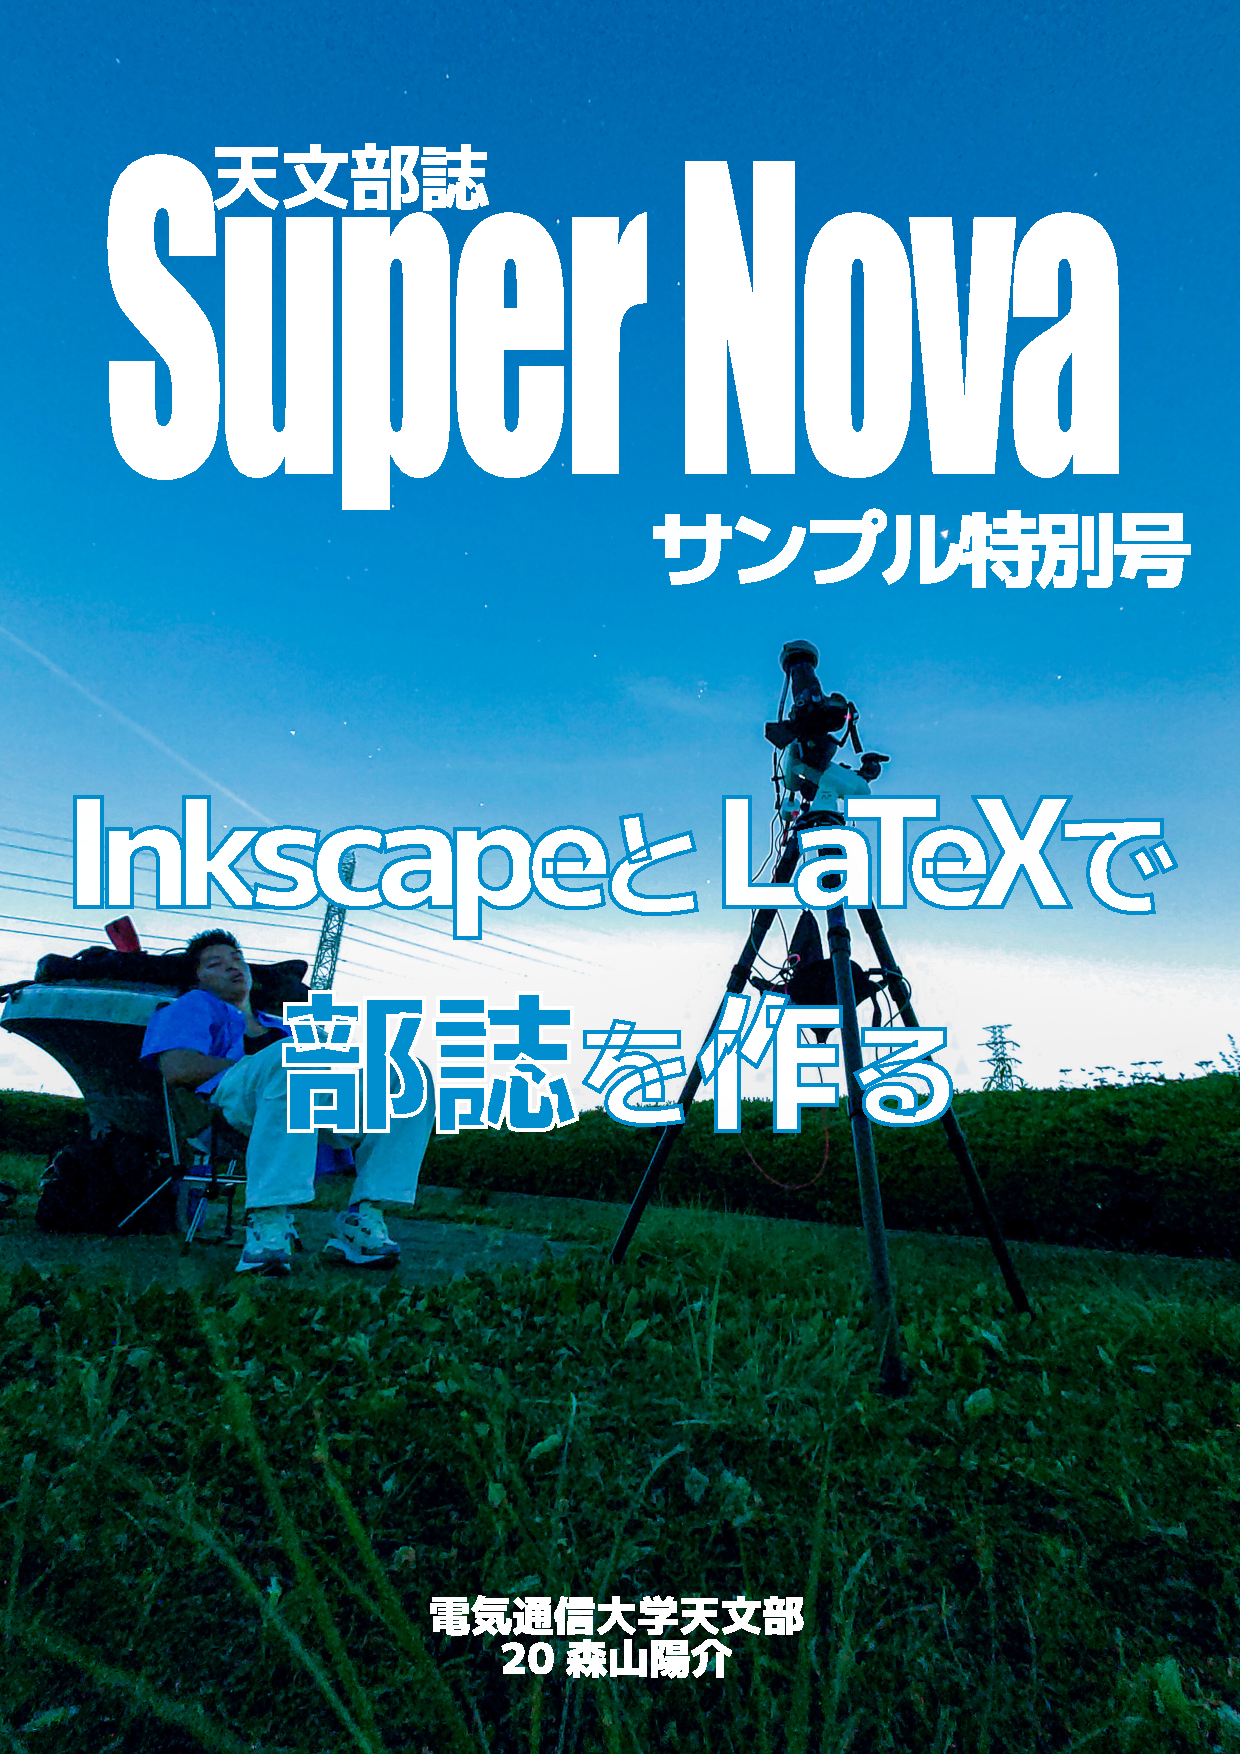
\includepdf[noautoscale=true, fitpaper]{cover/20yy_sample_supernova_cover.pdf} %表紙
\frontmatter
\setcounter{page}{1} %ページカウンタのセット
\subfile{sections/goaisatu} % ご挨拶ページ
\setcounter{tocdepth}{1} % 目次に表示する見出しの深さ指定 0:chapter 1:section 2:subsection 3:subsubsection
\tableofcontents % 目次
\cleartooddpage% 奇数ページまでジャンプ

\mainmatter
%%%%%%%%%   ここから本編   %%%%%%%%
% \subfile{hogehoge} % hogehoge.texを読み込む
\subfile{sections/contents}

%%%%%%%%   付録・編集後記   %%%%%%%%
\appendix
\subfile{sections/appendix} % 付録

\backmatter % あとがき、編集後記はこの下に
\subfile{sections/kouki} % 編集後記
%\printbibliography[title=参考文献]
%\addcontentsline{toc}{chapter}{参考文献}
% \includepdf[noautoscale=true, fitpaper]{cover/20yy_xxxx_atogaki.pdf}
\cleardoublepage
\cleartoevenpage % 奇数ページまでジャンプ
\includepdf[noautoscale=true, fitpaper]{cover/20yy_sample_supernova_cover_back.pdf} % 裏表紙
\end{document}
